% This is sigproc-sp.tex -FILE FOR V2.6SP OF ACM_PROC_ARTICLE-SP.CLS
% OCTOBER 2002
%
% It is an example file showing how to use the 'acm_proc_article-sp.cls' V2.6SP
% LaTeX2e document class file for Conference Proceedings submissions.
% ----------------------------------------------------------------------------------------------------------------
% This .tex file (and associated .cls V2.6SP) *DOES NOT* produce:
%       1) The Permission Statement
%       2) The Conference (location) Info information
%       3) The Copyright Line with ACM data
%       4) Page numbering
%
%  However, both the CopyrightYear (default to 2002) and the ACM Copyright Data
% (default to X-XXXXX-XX-X/XX/XX) can still be over-ridden by whatever the author
% inserts into the source .tex file.
% e.g.
% \CopyrightYear{2003} will cause 2003 to appear in the copyright line.
% \crdata{0-12345-67-8/90/12} will cause 0-12345-67-8/90/12 to appear in the copyright line.
%
% ---------------------------------------------------------------------------------------------------------------
% It is an example which *does* use the .bib file (from which the .bbl file
% is produced).
% REMEMBER HOWEVER: After having produced the .bbl file,
% and prior to final submission,
% you need to 'insert'  your .bbl file into your source .tex file so as to provide
% ONE 'self-contained' source file.
%
% Questions regarding SIGS should be sent to
% Adrienne Griscti ---> griscti@acm.org
%
% Questions/suggestions regarding the guidelines, .tex and .cls files, etc. to
% Gerald Murray ---> murray@acm.org 
%
% For tracking purposes - this is V2.6SP - OCTOBER 2002


\documentclass[12pt]{article}

\setlength{\oddsidemargin}{0in}
\setlength{\evensidemargin}{0in}
\setlength{\topmargin}{0in}
\setlength{\headheight}{0in}
\setlength{\headsep}{0in}
\setlength{\textwidth}{6in}
\setlength{\textheight}{9in}
\setlength{\parindent}{0in} 

\usepackage{graphicx} %For jpg figure inclusion
\usepackage{times} %For typeface
\usepackage{epsfig}
\usepackage{color} %For Comments
%\usepackage[all]{xy}
\usepackage{float}
%\usepackage{subfigure} 
\usepackage{hyperref}
\usepackage{url}
\usepackage{parskip}

%% Elena's favorite green (thanks, Fernando!)
\definecolor{ForestGreen}{RGB}{34,139,34}
\definecolor{BlueViolet}{RGB}{138,43,226}
\definecolor{Coquelicot}{RGB}{255, 56, 0}
%Uncomment this if you want to show work-in-progress comments
\newcommand{\comment}[1]{{\bf \tt  {#1}}}
% Uncomment this if you don't want to show comments
%\newcommand{\comment}[1]{}
\newcommand{\emcomment}[1]{\textcolor{ForestGreen}{\comment{Elena: {#1}}}}
\newcommand{\todo}[1]{\textcolor{blue}{\comment{To Do: {#1}}}}
\newcommand{\pscomment}[1]{\textcolor{Coquelicot}{\comment{Paul: {#1}}}}
\newcommand{\mmcomment}[1]{\textcolor{magenta}{\comment{Max: {#1}}}}
\newcommand{\escomment}[1]{\textcolor{BlueViolet}{\comment{Emma: {#1}}}}
\newcommand{\alcomment}[1]{\textcolor{red}{\comment{Lemmon: {#1}}}}

%%%%%%%%%%%%%%%%%%%%%%%%%%%%%%%%%%%%%%%%%%

\begin{document}
\pagestyle{plain}
%
% --- Author Metadata here ---
%\conferenceinfo{WOODSTOCK}{'97 El Paso, Texas USA}
%\setpagenumber{50}
%\CopyrightYear{2002} % Allows default copyright year (2002) to be
%over-ridden - IF NEED BE. 
%\crdata{0-12345-67-8/90/01}  % Allows default copyright data
%(X-XXXXX-XX-X/XX/XX) to be over-ridden. 
% --- End of Author Metadata ---

\title{Developing Beginner-Friendly User Interactions for the Clojure Programming Language}
%\subtitle{[Extended Abstract \comment{DO WE NEED THIS?}]
%\titlenote{}}
%
% You need the command \numberofauthors to handle the "boxing"
% and alignment of the authors under the title, and to add
% a section for authors number 4 through n.
%
% Up to the first three authors are aligned under the title;
% use the \alignauthor commands below to handle those names
% and affiliations. Add names, affiliations, addresses for
% additional authors as the argument to \additionalauthors;
% these will be set for you without further effort on your
% part as the last section in the body of your article BEFORE
% References or any Appendices.

\author{
Henry Fellows, Aaron Lemmon, Max Magnuson, \\
	Emma Sax, Paul Schliep, and Elena Machkasova \\
Computer Science Discipline \\
University of Minnesota Morris\\
Morris, MN 56267\\
fello056@umn.edu, lemmo031@umn.edu, magnu401@umn.edu, \\
	saxxx027@umn.edu, schli202@umn.edu, elenam@umn.edu
}
\date{}
\maketitle
\thispagestyle{empty}

\section*{\centering Abstract}
The abstract
\escomment{Is this supposed to be the abstract that we submitted? The
  one that's three paragraphs long?}
\emcomment{No, usually it's different from the abstract submitted for
  review. An abstract is usually written when the paper is nearly
  finished.}

\newpage
\setcounter{page}{1}

\section{Introduction and Background}\label{sec:intro}
\subsection{Overview of Clojure}\label{sec:clojure}
%\emcomment{Emma - many thanks for getting things started! Below are
%  comments. The majority of them refer to making this material
  %understandable to the target audience (i.e not using terms that
  %CSci undergrads typically don't know. Otherwise things are well
  %organized and well written.}
  
  
Clojure, developed in 2007 by Rich Hickey~\cite{Hickey:2008}, is a dynamic, functional
programming language in the Lisp family. Dynamic typing means that Clojure does not try to specifically associate
values with a type, but rather tries to figure out what type a value is at runtime.
\emcomment{need to be more precise here; also probably need to explain what ``functional'' means.}
%\emcomment{``dynamic'' refers to ``dynamically typed''} 
%\emcomment{Use simpler, more concrete terminology: there are many ways
  %in which JVM can be utilized. Probably need to explain that the JVM
  %is Clojure interpreter, mention and explain REPL somewhere in this paragraph.}
%\emcomment{Need to explain what you mean by dynamic}
Clojure utilizes the Java Virtual Machine (JVM) as an interpreter, and Clojure code compiles to JVM bytecode.
This setup offers easy 
%\emcomment{accessibilty?} 
accessibility of Java frameworks. The Clojure REPL
\emcomment{what does REPL stand for?} 
is another easy way to get acquainted \emcomment{to interact with Clojure?} with Clojure. A REPL is an interactive shell program that takes single 
expressions, evaluates them, and returns the result to the user. The REPL allows users to see immediate results
 and respond easily and quickly. For any programmer, the use of the REPL 
is highly advised and can make programming in Clojure much simpler. 
\emcomment{explain why?}
%\emcomment{This wouldn't make any sense to the target audience and is
  %not needed (perhaps with the exception of multithreading:}
%including optional type hints
%and type inference and easy multithreading options. All the while,
%Clojure remains completely dynamic.  
%\emcomment{This is a strange wording: what does it mean to ``remain''
 % in this context? And you already said it was dynamic.}

Because Clojure is a functional language, it puts strong emphasis on
immutable data types. An immutable data type means data cannot 
%\emcomment{data cannot be changed, not data types}
be changed, unlike in %\emcomment{in? Also, why ``many'' and not all of
  %them?}
  imperative programming languages. When using
Clojure, in order to change a data item, an entirely new data item
must be made. Immutable data types help prevent side effects in the program. 
A side effect is when a function alters memory
or interacts outside of its scope instead of \emcomment{or in addition to} returning a value. Side
effects can make debugging or resolving errors or failures more
difficult. This is because when a function interacts with other
functions \emcomment{with other parts of a program}, when it is not supposed to, any issues in the 
code can be spread out throughout the program. The reduction of side
effects means problems with the code are easier to find and fix.
Because of this, immutable data types are practical for novice
programmers.
%\emcomment{I would first explain what side
  %effects are, and only then why they complicate things for novice
  %programmers}
 
Clojure, like other Lisp languages, uses prefix notation. This means
that function calls use parenthesis, followed by the function name,
and then any parameters: 
\begin{verbatim}
	(<function-name> <argument 1> <argument 2>)
\end{verbatim}

An example of this can be seen through a built-in mathematical function, addition:
% \emcomment{All functions, including built-in mathematical functions, use this form? ``Even'' implies that somehow this is unexpected.} built-in functions, such as mathematical functions, use this form:
\begin{verbatim}
	(+ 5 5)
	-> 10
\end{verbatim}

Note that \texttt{->} indicates the result of computations in the Clojure interpreter.
%\emcomment{We indicate the result of computations in Clojure
  %interpreter as \texttt{->} -- plus we need to explain REPL and
  %interpreter.}

%\emcomment{I don't think we need syntax for interop. I would comment
 %out the example for now.}
Clojure also has easy accessibility to Java functions and Java
interoperability. This means that any Java method can be called just
like normal Clojure functions.
%\begin{verbatim}
%	(.methodName object *arguments)
%\end{verbatim}

%\emcomment{Thsi is true, but probably not useful for our readers}
%As well as the use of Java methods, Clojure can also use macros, Java
%utilities, concurrency and multithreading, and even certain Java
%objects to enhance the abilities of using Clojure. 

%\emcomment{before we get into anonymous functions, we need to show how
%to define regular functions (general syntax and a couple of examples)}
When a program needs to use a single value or function, it can be helpful to define it under a variable name
so that it's easier to access throughout the program. 
\emcomment{I don't think we need to explain why people name functions} 
Using the command \texttt{def} or \texttt{defn}, we
can define functions and variables \emcomment{this is a confusing way of saying it, especially because what you are showing is not a function. How about just talking about defining variables? (and technically functions are values anyway, just liek numbers and strings }:
\begin{verbatim}
	(def mystring "Hello World")
	mystring
	-> "Hello World"
\end{verbatim}

In the above example, we define a string to be \texttt{"Hello World"}. This way, whenever we utilize 
%\emcomment{I would avoid ``call'' here since calling is for functions} 
\texttt{mystring}, the string we bound to the variable name will be returned. Here is an example of using \texttt{defn} \emcomment{need to say that defn is used for defining functions} :
\begin{verbatim}
	(defn increment-number [number] (+ number 1))
	(increment-number 2)
	-> 3
\end{verbatim}

In this example, we saved \emcomment{define} a function that takes a number and increments it by adding 1 to it \emcomment{returns that number incremented by 1}. 
In any function, the 
function name is the word after the \texttt{defn}, the pieces in the square brackets after the function name indicate 
the arguments that the function takes in, and what follows is the body, or what the action of the function is \emcomment{the expression that the function returns ("action" sounds imperative)}. 
%\emcomment{the expression returned by the function? ``does'' has imperative flavor}

Now let us say that we have a program where we want to use a function, but only once. This means that we do not
necessarily need to define it with a name because Clojure supports anonymous functions. Anonymous functions allow 
programmers to quickly make
% \emcomment{not sure what you mean by``rare'' here. Those that aren't predefined?}  
functions when needed. 
However, since these functions are not  stored, the program would not be able to use them more than once. 
%\emcomment{call them?} by name after the usage. 
The following example is of the same increment-number function as above, but implemented anonymously: 
\begin{verbatim}
	(fn [number] (+ number 1))
\end{verbatim}
\emcomment{Give an example of using an anonymous function}

%In anonymous functions, anything in the brackets that is following the
%\texttt{fn} is arguments. 
%\emcomment{and in regular functions as well} 
%After the arguments in \texttt{[]}, is the
%body. If the program wanted to be able to call this function multiple
%times, it would make more sense to simply put a \texttt{def} with a
%name in front: 
%\emcomment{It's not quite that: firstly, it's defn, and not def, but
 % you also need to explain where the function name is}
%\begin{verbatim}
%	(def increment-number [number] (+ number 1))
%\end{verbatim}

%Now, the program can call this function any time by using the name \texttt{increment-number}.

Clojure also has a variety of different types of data structures. All 
of Clojure's collections are immutable, which means that the data within the structures cannot be modified. 
%\emcomment{I wouldn't go into persistent, just talk about immutable.}
%This means that the data in the structures cannot be modified, and that each
%structure preserves the previous version of itself. 
The different types of structures Clojure uses are lists (denoted by \texttt{()}),
sets (denoted by \texttt{\#\{\}}), vectors (denoted by \texttt{[]}),
and hashmaps (denoted by \texttt{\{\}}). The first three types of data
structures listed can contain any number, including \texttt{nil} (Clojure's equivalent of \texttt{null} or nothing), of 
values of any type (a data structure is untyped, which means values of different types can be  
%\emcomment{too informal, rephrase} if types of values in one structure
mismatched):
\mmcomment{I think that the above sentence should make it more clear that a collection may contain any data type. Maybe, don't mention numbers and stick to data types?}
\emcomment{agree}
%\emcomment{don't use the word ``normal'' in a research paper} data structures: 
\begin{verbatim}
	(1 2 "foo" :a 9 "bar")
\end{verbatim}

%\emcomment{I am not sure which of data structures we will actually need; we
  %never defined keywords, and I am not sure we will need those (but if
  %we do, we will need to explain them). We will definitely need
  %vectors and lists and hashmaps. Sets probably not.}

%They \emcomment{Not sure what ``they'' referes to; most structures can
%hold any amount (any number, to be more precise) of values, nil isn't
%explained, and probably needs to 
%be, but I am not sure; nil isn't an amount of anything.} can hold any
%amount, including \texttt{nil}, of values of any type 
%\emcomment{we need to mention earlier that all data structures are
 % untyped: not unique to hashmaps}
%(a data structure is untyped, which means it does not care if
%types of values in one structure as mismatched).

However, hashmaps are unique in the fact that a hashmap is a collection of key-value pairs: 
\begin{verbatim}
	{key value, key value, key value}
\end{verbatim}

An example 
%\emcomment{why ``realistic''? Just an example. What you are showing above is abstract syntax} 
 would look something like:
\begin{verbatim}
	{:a 1, :b 2, :c 3}
\end{verbatim}
%\emcomment{It's unclear from just the syntax what it means to be a
%  collection of key/value pairs.}

%\emcomment{I would first introduce keywords and then explain that they are typically used as keys}
\emcomment{Introduce keywords as a datatype before you first use them in an example (perhaps before collections)}
Keywords are a simple indicating word that have a colon in front. Examples of keywords can be seen in the
above hashmap: \texttt{:a}, \texttt{:b}, and \texttt{:c}. Keywords, such as the ones above,
are often used as keys within hashmaps. The value is the second piece of key-value pair,
and each value is bound to each key. In the above example, \texttt{:a} is bound to \texttt{1}, \texttt{:b}
is bound to \texttt{2}, and \texttt{:c} is bound to \texttt{3}.
%.  Keywords, such 
%In hashmaps, usually keywords, indicated by a colon in front of a
%simple indicating word, are used as keys, and the value is what the
%key is bound to. 
%\emcomment{keys aren't pointing to anything, they are bound to something}
%In the hashmap above, the keywords are


Just like variables and values, data structures can also be bound to a
variable name: 
\begin{verbatim}
	(def myhashmap {:a 1 :b 2 :c 3})
	myhashmap
	-> {:a 1, :b 2, :c 3}
\end{verbatim}

%This enables the data structures to be called, traversed, etc by the
%use of a single name. \emcomment{I am not sure this addds anything; an
%example would be better.}

\subsection{Overview of ClojurEd project}\label{sec:project}

\section{Error Messages}\label{sec:errors}

\subsection{Current error messages in Clojure}\label{sec:currentem}
Error messages are an important part of programming since they are the main source of communication between a user and the system when an error occurs in the program.
Error messages are especially important for introductory programmers who have had little to no experience with troubleshooting problems \emcomment{programs?}.
These error messages need to be user friendly to provide value to the introductory students.
For error messages to be useful, they should provide helpful and easy to understand information that can be used to resolve issues. 
\emcomment{The two sentences are very similar and should be merged}

Error messages in Clojure are not particularly useful for introductory programmers because they do not provide information that can help lead a student to fixing the error.
Also, Clojure error messages are typically complex because they originate from the underlying Java interpreter (the JVM), which many \emcomment{most} novice programmers will be unfamiliar with.
Below is an example of an error message in Clojure that might be unhelpful or unintuitive for an introductory student:

Code Sample:
\emcomment{Consider the following (erroenous) code fragment:}
\begin{verbatim}
(defn squareThis (* input input))
\end{verbatim}

In this code sample, the programmer is attempting to create a function \texttt{squareThis} which will take a number and return the square of its value.
However, the programmer forgot to declare that \texttt{input} should be a parameter.
In Clojure, function declarations typically require a vector containing the declared parameter names.
The resulting error message is: 
\begin{verbatim}
IllegalArgumentException Parameter declaration * should be 
a vector 
clojure.core/assert-valid-fdecl (core.clj:6842)
\end{verbatim}
It does provide key words that could lead the programmer to fixing the issue such as \texttt{Parameter} and \texttt{vector}.
However, the error message also includes information that a new programmer might find intimidating or confusing such as 

\noindent
\texttt{clojure.core/assert-valid-fdecl (core.clj:6842)}.



When writing functions in Clojure, a vector of arguments should immediately follow the name of the new function. 
\emcomment{The previous sentence creates an awkward flow. Maybe "the error can be corrected by placing a vector of inputs, in this case containing a single input, right after the function name"?}
Here is an example of the code above after corrections:
%Corrected Code:
\begin{verbatim}
(defn squareThis [input] (* input input))
\end{verbatim}

In the next example, the programmer is attempting to return a new hashmap with an added key-value pair.
The function \texttt{assoc} is generally used to make this happen.
\begin{verbatim}
(assoc :a 3 {:a 5, :b 8, :c 9})
\end{verbatim}

In this attempt, the programmer did not put the arguments for \texttt{assoc} in the correct order.
When using the function \texttt{assoc}, the hashmap should go before the new key and value.
The error message that results follows:

\begin{verbatim}
ClassCastException clojure.lang.Keyword 
cannot be cast to clojure.lang.Associative
clojure.lang.RT.assoc (RT.java:702)
\end{verbatim}

Since Clojure expects the first argument to be a hashmap and it is not, it unsuccessfully tries to cast the keyword \texttt{:a} into a hashmap.
This error message refers to \texttt{clojure.lang.Associative}, which is actually a Java interface.
\emcomment{it also refers to typecasting which is unfamiliar to Clojure users since Clojure is dynamically typed with no explicit type declarations.}
Referring to that interface may not be useful for Clojure programmers if they have little to no experience with Java or type hierarchies.
The error message is ineffective at explaining to the programmer that the underlying problem with their code was a misordering of arguments. Here is an example of the code above after corrections:
 
\begin{verbatim}
(assoc {:a 5, :b 8, :c 9} :a 3)
-> {:c 9, :b 8, :a 3}
\end{verbatim}

\emcomment{You might want to talk about the message transformations first, and then user scenarios used to test how well it works} 

\subsection{User scenarios}\label{sec:scenarios}

In order to better understand what our software users might encounter, we develop user scenarios detailing typical coding problems a new programmer might face.
To create these user scenarios, we developed solutions to common beginner programming exercises and purposefully introduced errors that a new programmer might make.
We then recorded the error messages that these solutions produced.
We also took note of the underlying cause of the errors so that we have a better idea of how to improve upon the error messages for our program.
We then took the same solution and ran it within our program to compare the error message our system produces against the one Clojure produces.  

These user scenarios showed us what the typical errors are a student will be running into when learning programming in Clojure for the first time.
For example, when a student first starts writing basic operations in Clojure, a typical mistake might be forgetting to put the function in front of the arguments, such as \texttt{(5 - 5)}, where it should be \texttt{(- 5 5)}. 
This produces a rather unhelpful error message: 

\begin{verbatim}
ClassCastException java.lang.Long cannot be cast to clojure.lang.IFn
user/eval769 (NO_SOURCE_FILE:1)
\end{verbatim}

\pscomment{What we learned from them scenarios}

\pscomment{Work in progress...}

\subsection{Error message transformations}\label{sec:transform}

Since standard Clojure error messages are generally unhelpful, we aim to replace many Clojure error messages with improved ones.
One way to accomplish this is to define functions with the same name as standard Clojure functions.
Within these definitions, we can do type checking on arguments passed in.
If the type checks find an error, our system displays a customized error message.
If no type errors are found, the arguments are passed on to the actual corresponding Clojure function.

Another way to replace Clojure error messages is to capture the thrown errors and rethrow our replacement messages.
We have a large collection of regular expressions that are checked against any Clojure error messages.
If a regular expression matches, important details from the original error message are captured and passed on to our replacement messages.


\subsection{Hints}\label{sec:hints}
\section{Technical Setup}\label{sec:technical}
In approaching error handling, there are many technical issues. First we need to figure out how to catch and process the errors. Then, we need to figure out how to integrate that system with the tools for managing Clojure projects. Throughout this process it is important to keep in mind the usability for introductory students. Therefore, we would like to abstract over as much as we can, while still providing a robust system for students to develop their Clojure projects.

Stuff to include:

Explain the difference between compilation and runtime and how that affects error messages.

Explain interaction with Repl and whole code compiling. \emcomment{be consistent with capitalization of REPL} 

Explain lazyness and its problem in error handling.

Diagram of how error handling works now, and how error handling works in our system.

Describe our process of error handling.

\emcomment{make it clear what's done and what's work in progress}

\subsection{Leiningen}
Leiningen \emcomment{reference, mention who developed it (or that it is an open source project)}  is a fully featured project manager that cleanly deals with dependencies as well as provides useful tools for developing projects. When a project is run in Leiningen, Leiningen will resolve all dependencies. For example, if your project requires a plugin, Leiningen will automatically retrieve, install, and apply that plugin to your code. After it has resolved the dependencies, Leiningen uses other tools to build, compile, and run the project. Leiningen makes running Clojure projects extremely simple. With Leiningen, it only takes one command to begin a new project, and it only takes one command to run a project. Because of the level of abstraction that Leiningen offers, we have decided that it is the best option for an introductory course.

While Leiningen is a very helpful tool, there are still some aspects that are challenging for introductory students. The most difficult of which is the interface. Leiningen uses the command line as its primary interface. The command line is both a distraction and a barrier to teaching the material in an introductory course. Therefore, we would like to abstract over the command line by using a graphical interface. This graphical interface would extend the simplicity of Leiningen while still providing the same functionality needed by students.

Leiningen is the primary tool in the Clojure community for handling Clojure projects.

\subsection{IDEs}
Currently we are looking into LightTable and NightCode as IDEs for the introductory course. 
\emcomment{references, a bit about each, a bit about why we are considering both}
Outline for the Section:
We are looking at LightTable or NightCode for our primary IDE.

Ideally we would like our system to be IDE independent. But we need to be mindful of the usability of the IDE.

We would like to use an IDE that will be actively developed because that means there is less for us to maintain.

\subsection{Implementing Error Handling}

\begin{figure}[h]
 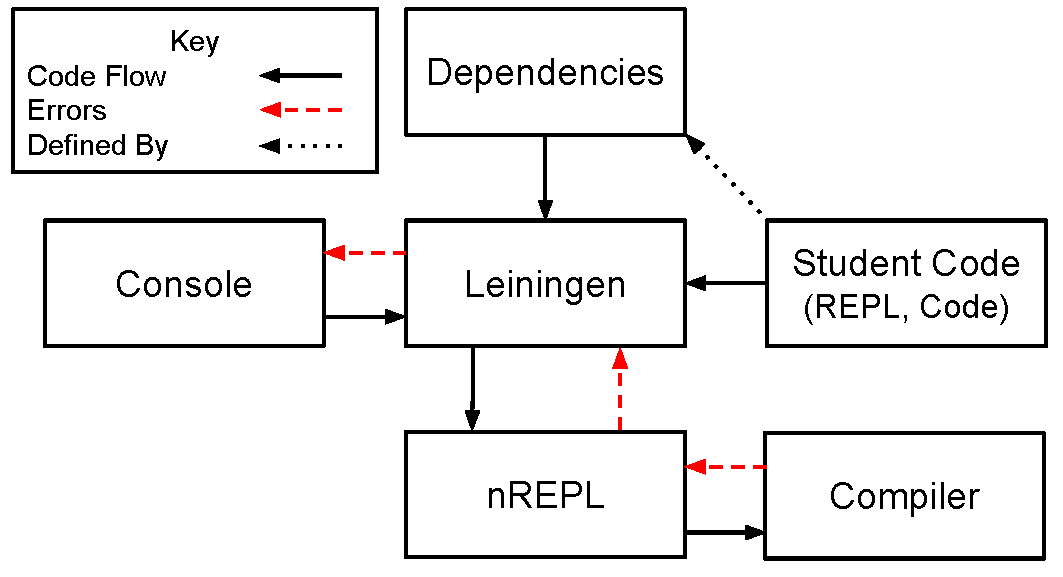
\includegraphics[width=12cm]{CurrentErrorHandling.pdf}
 \centering
 \label{fig:CurrentError}
\end{figure}

Stuff about figure \ref{fig:CurrentError}.

\begin{figure}[h]
 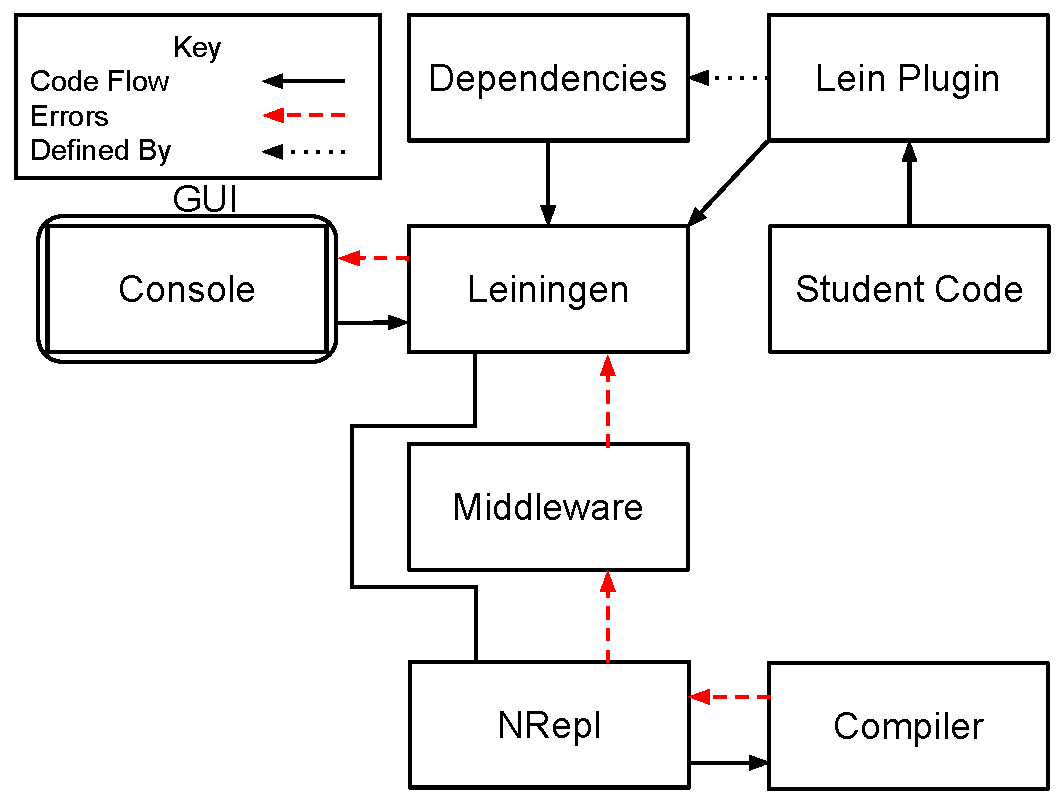
\includegraphics[width=12cm]{OurErrorHandlingSystem.pdf}
 \centering
 \label{fig:OurSystem}
\end{figure}

Stuff about figure \ref{fig:OurSystem}.

Outline for the Section:
We attempted to use IDE-specific plugins to handle error messages.

Then we tried Leiningen, and that didn't work out.

Now we are pretty sure that NRepl and its middleware is the key. Explain NRepl and middleware.

\section{Conclusions}\label{sec:conclusion}

\bibliographystyle{ACM}
\bibliography{mics2015}

% \section{References?}\label{sec:reference}
% \escomment{unsure if we actually put references directly into the
%   paper or not...}
% \emcomment{Emma - Don't worry about it for now. Do you have a reference you
%   would like to add?}
% \escomment{I have a few links to websites I used, but I'm not sure what format I should use for preparing them properly}

% That's all folks!
\end{document}
